\chapter{\heiti In MAC OSX}
\section{\heiti{Startup}}

\noindent Download the SDK from 
\\{http://china.cypress.com/documentation/software-and-drivers/ez-usb-fx3-software-development-kit}
\\ \\
Uncompress the SDK file:FX3\_SDK\_MacOS\_v1.3.3.tar.gz
\\ \\ 
And uncompress the file:cyusb\_mac\_1.0.tar.gz
\\ \\
Open the `docs' folder, and refer to `cyusb\_mac\_user\_guide.pdf'. You can start from the Section 2.1.

\begin{enumerate}
\item Install the library `libusb'.
\item Enter the `lib' folder and run `make' command in the terminal. Then copy the `*.dylib' file to the \/usr\/local\/lib.
\item Copy the configs\/cyusb.conf to \/etc folder.
\item Uncompress the file we provided and enter the directory which just be generated and run `.\/cybulk\_writer 512' command in the terminal. A demo signal is generated by the device and you could see it on the oscilloscope.
\item If fail, you should use the `cybulk\_writer.c' we provided to replace the same file in the  `examples' directory and run `make' command in the terminal. You will get many executable files. Then run `.\/cybulk\_writer 512' command again.
\end{enumerate}

\section{\heiti{API Introduction}}

We also provide API written in Python. The filename is `macosx\_pulse\_api.py'. Before you running the script, you must install python interpreter and package `numpy'. The Python script use the program `cybulk\_writer' to download data to the device. So they must exist in the same folder.
\\
\indent For the example to use the Python script, please refer to the functions `delay\_chain\_test' and `random\_pulse\_test' in the script. You can also run the script in the terminal. If all is configured well, the device will output signal.
\\
\indent We provide 3 API functions for the user: PB\_type\_program, start and stop. For more information, please refer to the comment in the function.
\\

Parameter for the function `PB\_type\_program':

\vspace{0.2cm}
\begin{table}[H]
%\begin{table}[!htbp]
\normalsize
%\caption{}
%\rowcolors{2}{gray!10}{gray!10}
\begin{tabular}{|m{6.5cm}<{\centering}|m{7cm}<{\centering}|}
%\begin{tabular}{p{0.5\textwidth}|p{0.5\textwidth}}
% \rowcolor{blue!50}
\hline Parameter Type & List[List[String, Float]...]
\\ 
\hline Example 1 & [['00001111', 10.0], ['11110000', 10.05]] 
\\ 
\hline Example 2 & [['10000000', 10.0], ['11000000', 0.05], ['01000000', 15.0]] \\\hline
\end{tabular}
\end{table}

\begin{figure}[ht]
\centering
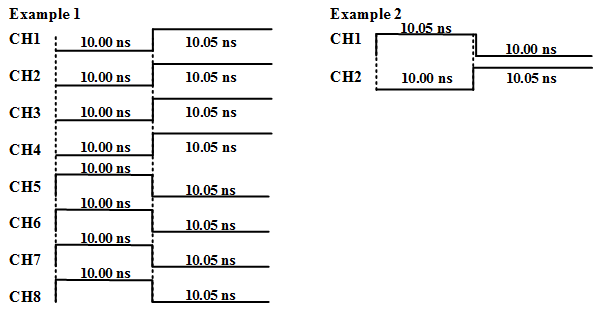
\includegraphics[height=6cm]{pulse_example_mac}
\caption{Example waveform}
\label{pulse_example_mac}
\end{figure}

\indent API calling example:

\begin{figure}[ht]
\centering
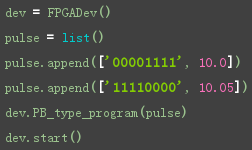
\includegraphics[height=4cm]{program_example_mac}
\caption{Program example}
\label{program_example_mac}
\end{figure}


\section{\heiti{Understand the Data Structure of the Pulse Sequence}}
\indent We use 10 bytes (80-bit) to describe a pulse with high level and low level. Each 80-bit data includes 32-bit high level time data, 32-bit low level time data, 5-bit leading edge delay data, 5-bit trailing edge delay data, and 6 reserved bits. 

\begin{table}[H]
\centering
\normalsize
\begin{tabular}{|m{3.5cm}|m{3.5cm}|m{0.5cm}|m{1cm}|m{0.5cm}|m{1cm}|}
% \rowcolor{blue!50}
\hline 32-bit & 32-bit & \qquad & 5-bit & \qquad & 5-bit \\\hline
\end{tabular}
\end{table}

\indent The least bit of the 32-bit data represents 0.625 ns for high level time or low level time. And the 5-bit data adjust the edge of the pulse with 50 ps resolution.
\indent A complicated pulse sequence consists of many 10 bytes elements. By utilizing the different storage space of DDR3, it can define arbitrary pulse sequence freely.